\section{Results and uncertainty}
% Original presentation frame 18
\begin{frame}[t,shrink=5]{Structured propagators reduce the observed endpoint error, but the numerical ranking is descriptive}
\begin{center}\begin{adjustbox}{max width=\linewidth}
\begin{tabular}{lrrrr}\toprule
Model & $\epsilon_{\mathrm{rel}}$ & SW & Bias norm & $\tau$ [ms/sample]\\\midrule
CVAE only, no propagation & 0.367 & 0.0096 & -- & --\\\midrule
Transformer, no window & 0.681 & 0.087 & 17.337 & 18.74\\
Transformer, $w=1$ & 0.650 & 0.026 & 52.389 & 14.35\\
Windowed Transformer ($w=8$) & 0.534 & 0.022 & 50.414 & 12.01\\
CVAE--GNO & 0.511 & 0.014 & 0.376 & 2.338\\\bottomrule\end{tabular}
\end{adjustbox}\end{center}\begin{columns}[T,onlytextwidth]
\begin{column}{0.49\textwidth}
\begin{block}{Global model comparison}
GNO present the lowest observed relative histogram and sliced-Wasserstein errors on the common held-out endpoint test set. Within the common neural benchmark, GNO is about eight times faster than global TF, under same hardware conditions.
\end{block}

\end{column}
\begin{column}{0.49\textwidth}
\begin{block}{Error quantification}
The CVAE--GNO error includes the pre-existing CVAE representation loss. Further uncertainty quantification is needed to test the accuracy and reliability of the learned propagation map.
\end{block}

\end{column}
\end{columns}

\sources{Transport metric: \parencite{peyre2019transport}.}

\end{frame}

% Original presentation frame 19
\begin{frame}[t,shrink=5]{A separate statistics head tests whether normalized shape can be returned to physical coordinates}
\begin{columns}[T,onlytextwidth]
\begin{column}{0.64\textwidth}
\begin{center}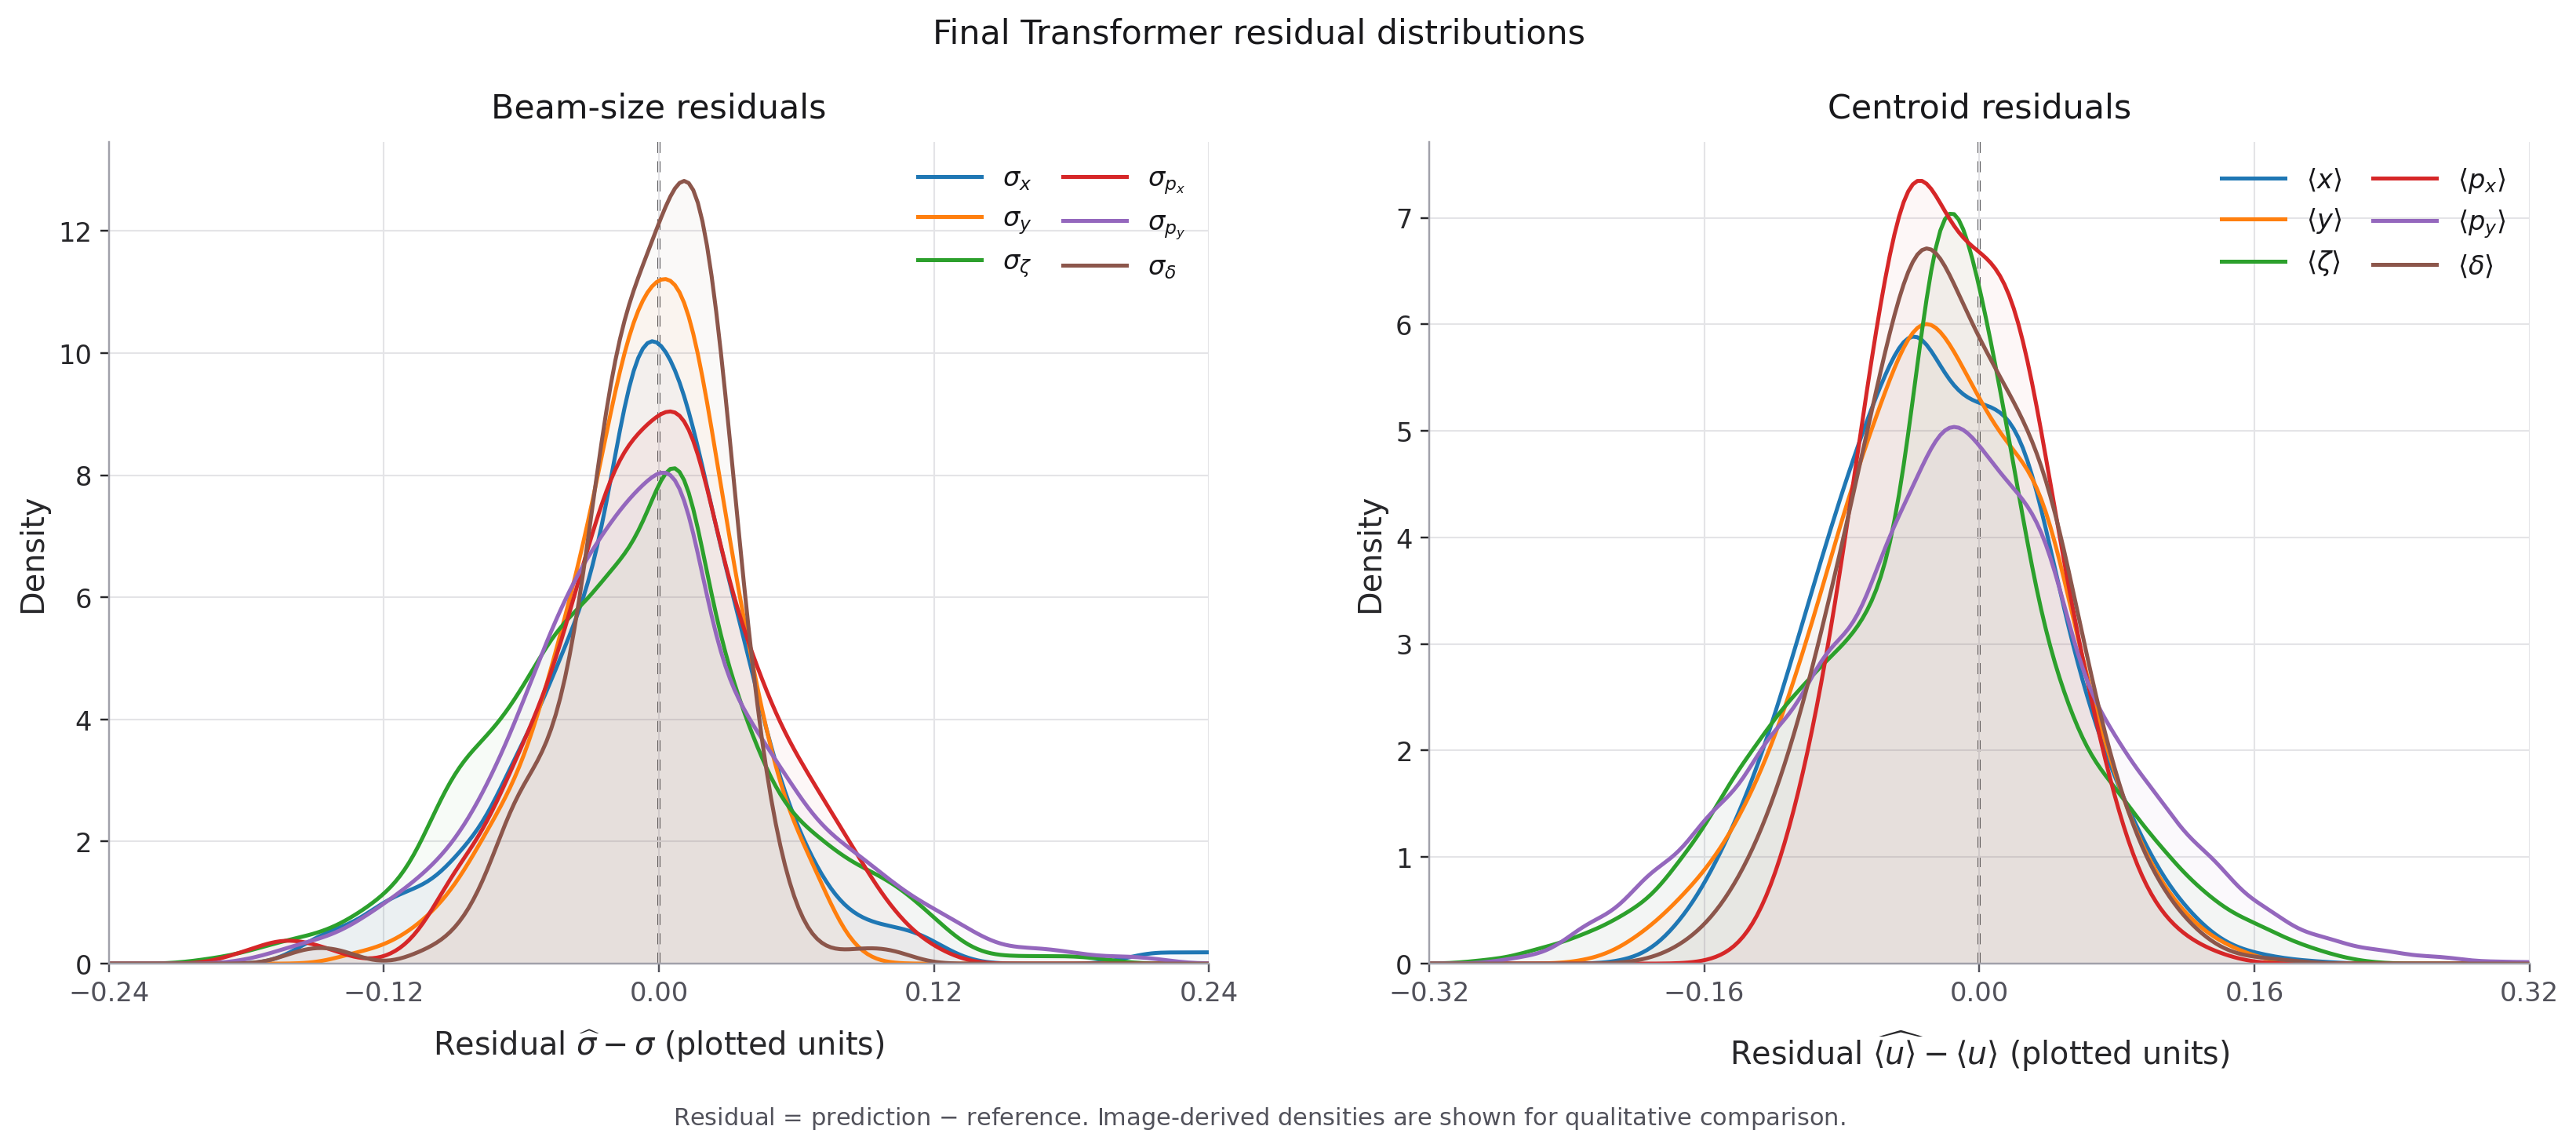
\includegraphics[width=\linewidth]{physical_statistics_stacked_residuals.png}\end{center}{\scriptsize Stacked residuals for the physical-statistics head, validation sample $s=3$. The model predicts the first two moments of each physical axis.\par}
\end{column}
\begin{column}{0.33999999999999997\textwidth}
\begin{block}{Physical head}
Unit-mass histograms use sample-adaptive support. The model predicts
\[\widehat q_N=(\widehat m_N,\widehat\sigma_N)\in\mathbb R^{12}\]
to recover physical axes and bin areas.

Centroids test first moments, coordinate-wise RMS spreads test physical extension. Only $\sigma_x$ and $\sigma_y$ are conventional transverse beam sizes under the stated optics assumptions.
\end{block}

\end{column}
\end{columns}

\end{frame}

% Original presentation frame 20
\begin{frame}[t,shrink=5]{For one fixed sample, prediction bias is much larger than the conditional latent spread}
\begin{columns}[T,onlytextwidth]
\begin{column}{0.63\textwidth}
\begin{center}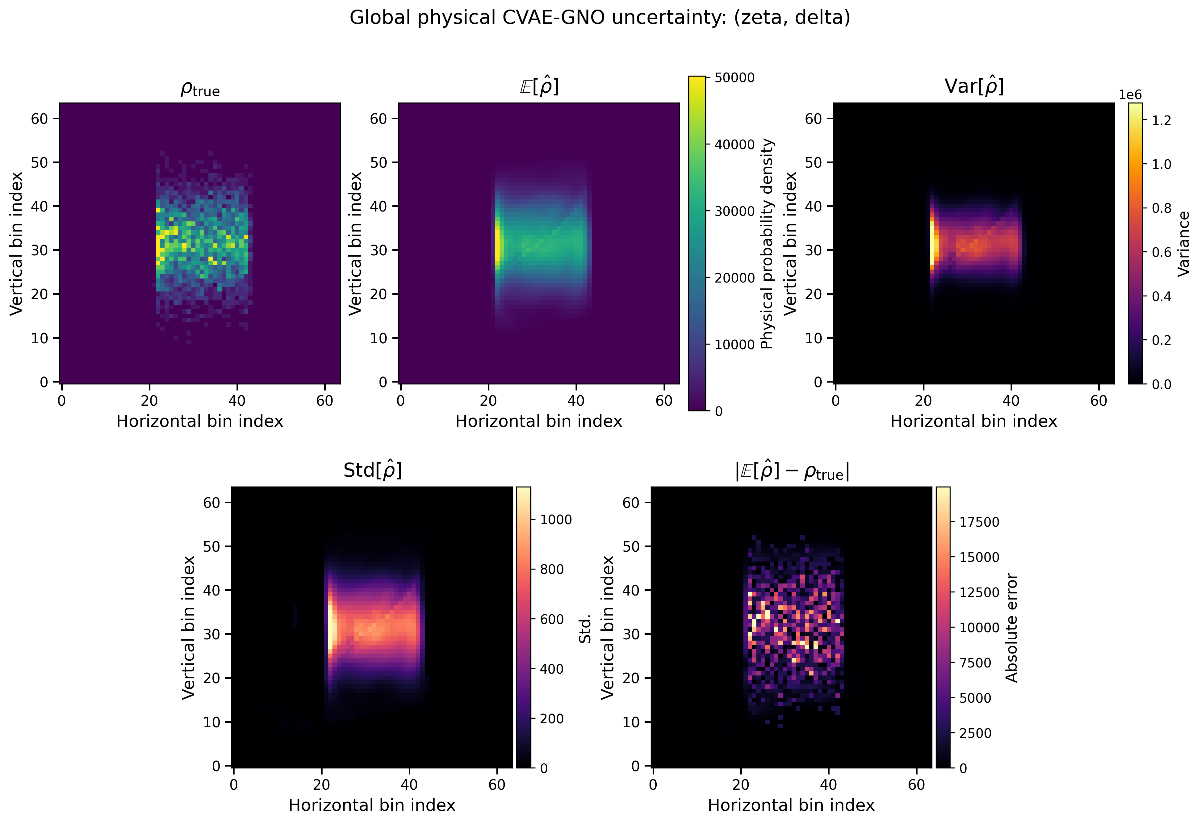
\includegraphics[width=\linewidth]{fixed_sample_latent_ensemble_diagnostics.png}\end{center}{\scriptsize $R=100$ draws for validation sample $s=3$, $(y,\delta)$: reference, ensemble mean, spread and discrepancy.\par}
\end{column}
\begin{column}{0.35\textwidth}
\begin{block}{Normalized mass}
\[\frac{\operatorname{mean}|\overline H-H_{\rm true}|}{\operatorname{mean}s_H}=19.6.\]
\end{block}
\begin{block}{Physical density}
\[\frac{\operatorname{mean}|\overline\rho-\rho_{\rm true}|}{\operatorname{mean}s_\rho}=55.5.\]The larger ratio reflects inverse-bin-area rescaling, not an independent uncertainty source.
\end{block}
{\scriptsize The ensemble is tightly clustered around a biased mean, increasing $R$ does not remove the systematic discrepancy.\par}
\end{column}
\end{columns}

\end{frame}

% Original presentation frame 21
\begin{frame}[t,shrink=5]{The held-out diagnostic remains under-dispersed even where absolute variance is largest}
\begin{columns}[T,onlytextwidth]
\begin{column}{0.68\textwidth}
\begin{center}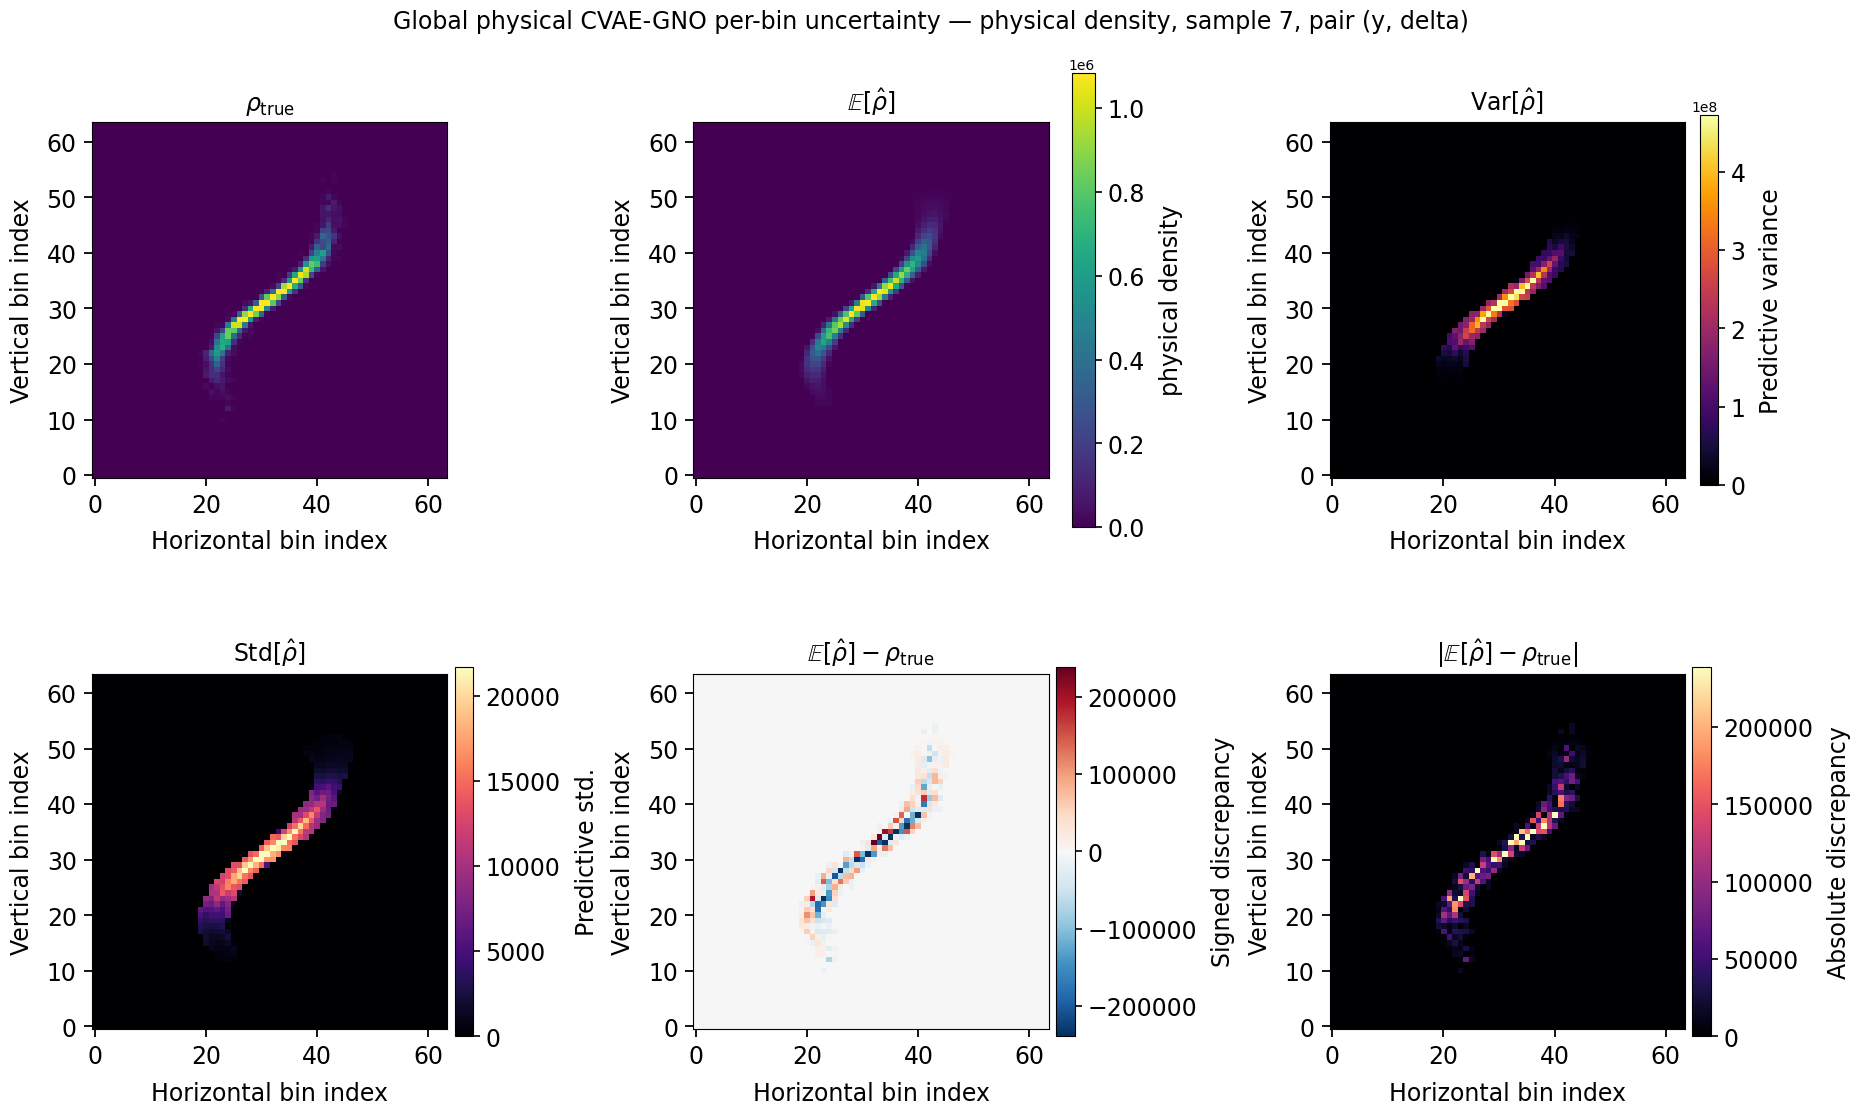
\includegraphics[width=\linewidth,height=54mm,keepaspectratio]{heldout_uncertainty_per_bin.png}\end{center}{\scriptsize $R=64$ stochastic passes for held-out sample $s=7$, $(y,\delta)$ projection.\par}
\end{column}
\begin{column}{0.29999999999999993\textwidth}
\begin{block}{Global comparison}
\[R_{\rm global}=\frac{3.487909\times10^3}{4.686791\times10^2}\simeq7.44.\]
\end{block}
\begin{block}{Highest-variance bin}
The ensemble mean overpredicts the reference by about $10.7\%$, latent spread is about $2.38\%$, so the mean lies approximately $4.5\sigma_{\rm latent}$ from the reference.
\end{block}

\end{column}
\end{columns}

\end{frame}

